\section*{Appendix I - Haar Wavelet}

A fundamental purpose of analysing functions such as the Fourier and wavelet functions are the reconstruction of signals from it’s decomposition.  Certain criteria or properties are therefore required for analysis functions.  

In Chapter \ref{c4_fourier}, the orthogonal properties of the Fourier transform equations was introduced.  In the case of wavelets the following properties ensue.  In addition to orthogonal properties, wavelets are required to perform localised analysis of a function. Hence, unlike their Fourier counterparts, they need to be bounded in time.  It is also seen that when the energy contained within the wavelet bases sum to zero (sometimes normalised to 1)i.e.
\begin{equation}
    E=\int_{-\infty}^\infty |x|^2dt=||x(t)||^2=0
    \label{app1_01_pwr}
\end{equation}

Then, such wavelet bases are orthonormal and the fundamental or scaling equation forms a recurrence relation which is a solution to the dilation equation as follows:
\begin{equation}
    \phi(t)=\sum_kc_k\phi(2t-k)
    \label{app1_02_dilation}
\end{equation}

Where $\phi(2t-k)$ is a contracted version of $\phi(t)$ shifted along the time axis by an integer step $k$ and factored by an associated coefficient $c_k$.  At the same time it is also observed that it is possible to setup this recurrence relation to becoming dyadic such that the sum of coefficients, $c_k$ equals $2$, i.e. $\Sigma_kc_k=2$. Haar, wavelets constitute the simplest of this family of wavelets.

The mother wavelet of the Haar wavelet has only two coefficients $c_0=c_1=1$ and is given by:
\begin{equation}
    \psi(t)=\phi(2t)+\phi(2t-1)
    \label{app1_03_mwavlet}
\end{equation}

Observe here that $c_0+c_1=2$, i.e. dyadic.  The solution to this recurrence equation and the resulting plot is given in Figure \ref{haar}. 

\begin{figure}
\centering
  % Requires \usepackage{graphicx}
  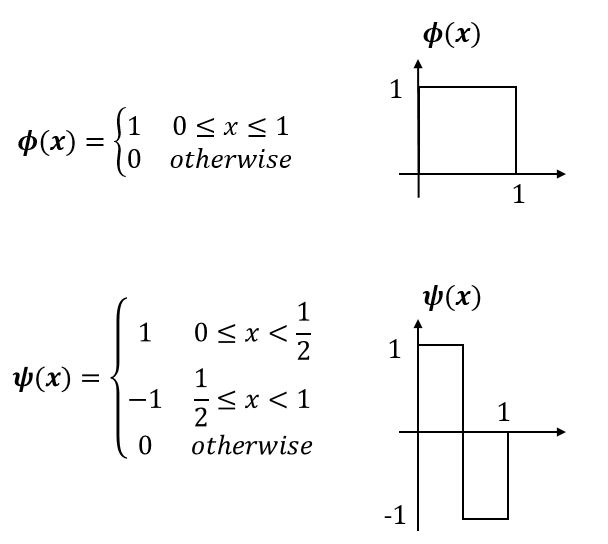
\includegraphics[width=14cm]{thesis/images/haar.png}\\
  \caption{Haar wavelet} \label{haar}
\end{figure}

Through multi-resolution analysis, the following reconstruction of the Haar wavelet is derived:

\begin{equation}
   \phi_{j,k}[n]=2^{j/2}\phi[2^jn-k]
    \label{app1_04_mres}
\end{equation}

The parameter $j$, controls the resolution of the signal reconstruction and the following wavelets and function representation are given in Figure \ref{multires}

\begin{figure}
\centering
  % Requires \usepackage{graphicx}
  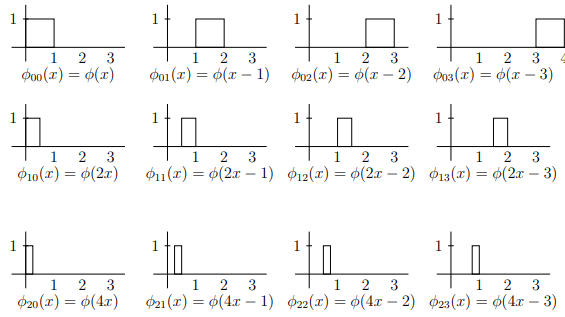
\includegraphics[width=14cm]{thesis/images/multires.png}\\
  \caption{Multi resolution analysis of Haar wavelets} \label{multires}
\end{figure}
